\documentclass[tikz,border=10pt]{standalone}
\begin{document}
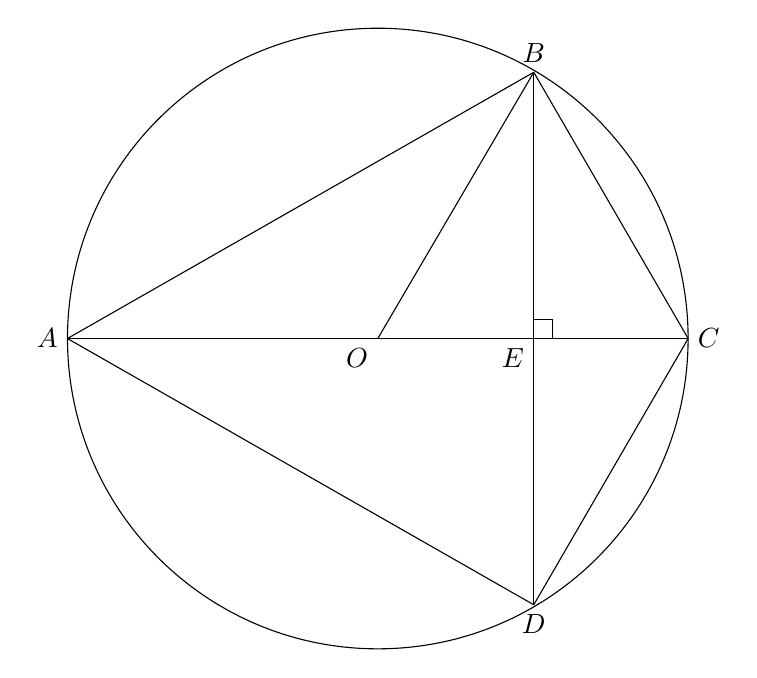
\begin{tikzpicture}[scale=0.02]
  \coordinate (O) at (0,0);
  \coordinate (A) at (-197,0);
  \coordinate (C) at (197,0);
  \coordinate (B) at (99,169);
  \coordinate (D) at (99,-169);
  \coordinate (E) at (99,0);

  \draw (O) circle (197);

  \draw (A) -- (B);
  \draw (B) -- (O);
  \draw (B) -- (C);
  \draw (B) -- (D);
  \draw (A) -- (D);
  \draw (D) -- (C);
  \draw (A) -- (C);

  \draw (99,0) -- (111,0) -- (111,12) -- (99,12);

  \node[above] at (B) {$B$};
  \node[left] at (A) {$A$};
  \node[right] at (C) {$C$};
  \node[below] at (D) {$D$};
  \node[below left] at (O) {$O$};
  \node[below left] at (E) {$E$};
\end{tikzpicture}
\end{document}
